\documentclass{beamer}

\mode<presentation> {
%\usetheme{default}
%\usetheme{AnnArbor}
%\usetheme{Antibes}
%\usetheme{Bergen}
%\usetheme{Berkeley}
%\usetheme{Berlin}
%\usetheme{Boadilla}
%\usetheme{CambridgeUS}
%\usetheme{Copenhagen}
%\usetheme{Darmstadt}
%\usetheme{Dresden}
\usetheme{Frankfurt}
%\usetheme{Goettingen}
%\usetheme{Hannover}
%\usetheme{Ilmenau}
%\usetheme{JuanLesPins}
%\usetheme{Luebeck}
%\usetheme{Madrid}
%\usetheme{Malmoe}
%\usetheme{Marburg}
%\usetheme{Montpellier}
%\usetheme{PaloAlto}
%\usetheme{Pittsburgh}
%\usetheme{Rochester}
%\usetheme{Singapore}
%\usetheme{Szeged}
%\usetheme{Warsaw}

% As well as themes, the Beamer class has a number of color themes
% for any slide theme.
%\usecolortheme{albatross}
%\usecolortheme{beaver}
%\usecolortheme{beetle}
\usecolortheme{crane}
%\usecolortheme{dolphin}
%\usecolortheme{dove}
%\usecolortheme{fly}
%\usecolortheme{lily}
%\usecolortheme{orchid}
%\usecolortheme{rose}
%\usecolortheme{seagull}
%\usecolortheme{seahorse}
%\usecolortheme{whale}
%\usecolortheme{wolverine}

%\setbeamertemplate{footline} % To remove the footer line in all slides uncomment this line
\setbeamertemplate{footline}[page number] % To replace the footer line in all slides with a simple slide count uncomment this line
\setbeamertemplate{navigation symbols}{} % To remove the navigation symbols from the bottom of all slides uncomment this line
\setbeamertemplate{headline}{} % Uncomment to remove navigation header
}

\usepackage{graphicx} % Allows including images
\usepackage{booktabs} % Allows the use of \toprule, \midrule and \bottomrule in tables
\usepackage[francais]{babel}
\usepackage[utf8]{inputenc}
\usepackage[T1]{fontenc}
\usepackage{transparent}
\usepackage{tikz}
\usepackage{tabularx}
\usepackage{hyperref}
\usepackage{fancyhdr}
\usepackage{float}
\usepackage{amssymb}
\usepackage{amsmath}
\usepackage[]{algorithm2e}
%\usepackage{media9}

\def\Put(#1, #2)#3{\leavevmode\makebox(0, 0){\put(#1, #2){#3}}}

\let\OLDtheorem=\theorem
\def\theorem{%
  \setbeamercolor{block title}{fg=white,bg=red!85!white}%
  \setbeamercolor{block body}{fg=black,bg=red!10!white}\OLDtheorem
}

\let\OLDdefinition=\definition
\def\definition{%
  \setbeamercolor{block title}{fg=white,bg=green!50!black}%
  \setbeamercolor{block body}{fg=black,bg=green!15!white}\OLDdefinition
}



%----------------------------------------------------------------------------------------
%	TITLE PAGE
%----------------------------------------------------------------------------------------

\title[Full title]{Une introduction à l'apprentissage automatique} % The short title appears at the bottom of every slide, the full title is only on the title page
%\subtitle{Lycée Gay-Lussac, Limoges}

\author{Eloïse BERTHIER}

\date{vendredi 8 mars 2019} 


\everymath{\displaystyle}

% show the table of contents before each section
\AtBeginSection[]
  {
    \ifnum \value{framenumber}>1
      \begin{frame}<beamer>
      \frametitle{Layout}
      \tableofcontents[currentsection]
      \end{frame}
    \else
    \fi
  }

\begin{document}

  \begin{frame}
  \titlepage 
  \Put(95, 10){
\includegraphics[width=0.4\linewidth]{images/logo.jpg}}
%\Put(230, 10){
\includegraphics[width=0.25\linewidth]{images/logo-ens.png}}

  \end{frame}
  
%\tableofcontents[sectionstyle=show/show, subsectionstyle=show/shaded/hide]
%  \tableofcontents[sectionstyle=show/show, subsectionstyle=hide]

% !TEX root=../main.tex

\begin{frame}{Quels outils pour le \textit{machine learning} ?}

\textit{Machine Learning} : l'étude scientifique des \textcolor{red}{\textbf{algorithmes}} et des modèles \textcolor{red}{\textbf{statistiques}} que les ordinateurs utilisent pour accomplir une tâche sans instruction explicite, mais plutôt en s'appuyant sur des motifs et de l'inférence.

\end{frame}


\begin{frame}{Un exemple simple : la régression linéaire}

\Put(210, -250){
\begin{minipage}{100pt}
On sait que la relation entre intensité et tension est linéaire : $$U = R I$$
On a collecté des données  \vspace{1em}  $(I_j, U_j)_{j \in \{1, ..., n \}}$.  On cherche à estimer la résistance $R$ inconnue.
\end{minipage}
}

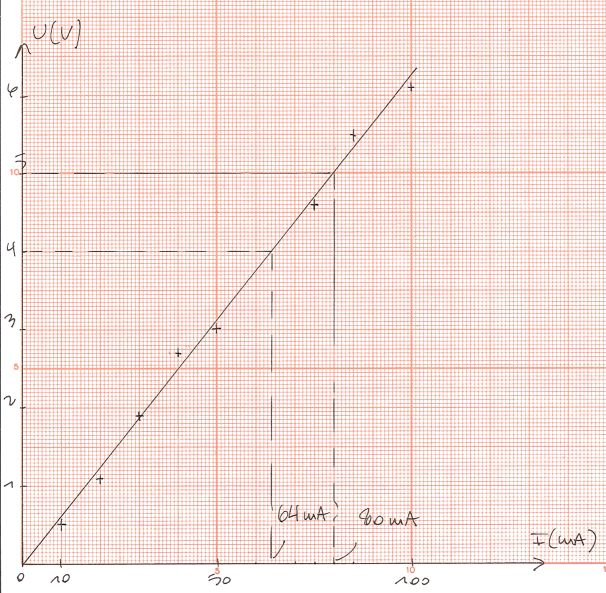
\includegraphics[width=7cm]{images/droite.jpg}

\end{frame}


\begin{frame}{Trois mots sur les statistiques}

$\bullet$ On suppose la relation entre intensité et tension linéaire : $U = R I$.

$\hspace{2em} \rightarrow$ C'est \textbf{un modèle} \textcolor{red}{\textbf{statistique}}.

\vspace{2em}

$\bullet$ On peut calculer explicitement le paramètre $\hat R$ estimé à partir des données. On peut même parfois obtenir une mesure d'incertitude.

$\hspace{2em} \rightarrow$ C'est \textbf{l'apprentissage} \textcolor{red}{\textbf{statistique}}.

\vspace{2em}

$\bullet$ Une fois $\hat R$ calculé, on peut l'utiliser pour prédire la tension à une nouvelle intensité $I_{new}$ : $$U_{new} = \hat R I_{new} $$
$\hspace{2em} \rightarrow$ C'est \textbf{l'inférence} \textcolor{red}{\textbf{statistique}}. 

\end{frame}


\begin{frame}{Comment construire un modèle statistique ?}

Choisir le bon niveau de complexité :

\includegraphics[width=11cm]{images/fit.png} 

\end{frame}

\begin{frame}{Comment construire un modèle statistique ?}

Solution : la validation croisée. Les données sont séparées entre :
\begin{itemize}
\item données d'entraînement
\item données de test
\end{itemize}

\includegraphics[width=11cm]{images/overfit.png} 

\end{frame}


\begin{frame}{Comment apprendre les paramètres d'un modèle ?}

\vspace{-2em}

\textbf{Régression linéaire en dimension $d$ :}

$\bullet$ Modèle : $y = \langle w, x \rangle + \varepsilon$, où $x \in \mathbb{R}^{d}, y \in \mathbb{R}$ et $w \in \mathbb{R}^d$.

 $\bullet$ Données d'apprentissage : $(x_i, y_i)_{i=1,...,n} \in (\mathbb{R}^d \times \mathbb{R})^n$.

$\bullet$ Minimisation de l'erreur d'apprentissage :  

 \hspace{1em} $\min_{w \in \mathbb{R}^d} \frac{1}{n} \sum_{i=1}^n \left( \langle w, x_i \rangle - y_i \right)^2 $

$\bullet$ Solution : $\hat w = (X^\top X)^{-1} X^\top y$

où $X = \begin{pmatrix}
   x_1^1 &  \hdots & x_1^d  \\
   \vdots &  \ddots &   \vdots  \\
   x_n^1 & \hdots  &x_n^d 
\end{pmatrix} $ et $y = \begin{pmatrix}
   y_1  \\
   \vdots  \\
   y_d
\end{pmatrix}$ 

\vspace{1.7em}


\Put(200, 40){\includegraphics[width=4.5cm]{images/xkcd.png} }

\hspace{1em} $\hookrightarrow$  \textcolor{red}{\textbf{Algèbre linéaire}}



\end{frame}

\begin{frame}{L'apprentissage supervisé : cas général}

Données d'apprentissage : $(X_i, y_i)_{i=1,...,n} \in (\mathcal{X} \times \mathbb{R})^n$.

Modèle : $y = f(x)$, pour un certain $f \in \mathcal{F}$.

Problème à résoudre pour l'apprentissage :
$$ \min_{f \in \mathcal{F}} \frac{1}{n} \sum_{i=1}^n \ell(f(x_i), y_i )+ \lambda \Omega(f)$$

\begin{tikzpicture}[overlay]
   \path[draw=magenta,thick,->]<1->  (2.9, 1) -- (2, 0);
   \path[draw=magenta,thick,->]<1->  (5, 0.6) -- (5, -0.5);
   \path[draw=magenta,thick,->]<1->  (7.2, 0.7) -- (8, 0);
\end{tikzpicture}

\Put(0, 0){ \textcolor{red}{\textbf{Optimisation}}}
\Put(120, -20){ Erreur}
\Put(200, 0){Régularisation}

\vspace{3em}

Trouver un modèle qui fait peu d'erreurs, et le plus simple possible.

\end{frame}


\begin{frame}{L'optimisation}

\Put(180, -100){
\begin{minipage}{120pt}
But : minimiser une fonction convexe.
\end{minipage}}


\Put(180, -150){
\begin{minipage}{120pt}
Trouver $u$ tel que $\forall v, f(u) \leq f(v)$.
\end{minipage}}

\vspace{-2em}
\includegraphics[width=5.5cm]{images/convex.png}

\vspace{-1em}
Fonction convexe : $\forall u, v, \lambda \in (0, 1), f((1-\lambda) u + \lambda v) \leq (1-\lambda) f(u) + \lambda f(v)$ 

\end{frame}



\begin{frame}{Un algorithme d'optimisation...}

L'\textcolor{red}{\textbf{algorithme}} le plus simple : la descente de gradient.

\includegraphics[width=8.5cm]{images/gd.png}

\vspace{2em}

Répéter jusqu'à convergence :
$ w \leftarrow w - \eta J^\prime(w) $

\end{frame}


\begin{frame}{... Des algorithmes d'optimisation}

\begin{itemize}
\item Gradient descent
\item Stochastic gradient descent
\item Coordinate gradient descent
\item Accelerated gradient descent
\item Averaged gradient descent
\item Subgradient descent
\item Proximal gradient descent
\item Conjugate gradient descent
\item Conditional gradient descent
\item Newton method
\item Quasi Newton methods
\item Alternative direction method of multipliers
\item Douglas-Rachford
\item ...
\end{itemize}

\Put(200, 250){+  versions distribuées}
\Put(200, 220){sur plusieurs machines}

\end{frame}


\begin{frame}{En pratique}

L'implémentation se fait majoritairement en \textcolor{red}{\textbf{Python}}, où la plupart des outils sont en \textit{open sourc}e et faciles d'utilisation.

\vspace{0.5em}

\includegraphics[width=11cm]{images/open_source.png}

\end{frame}

\begin{frame}{En quelques lignes de code}


\includegraphics[width=5cm]{images/sklearn.png}

\Put(150, 150){\includegraphics[width=6.2cm]{images/keras_code.png}}

\Put(150, 10){Réseau de neurones}

\vspace{-1.3em}
Régression linéaire

\end{frame}

%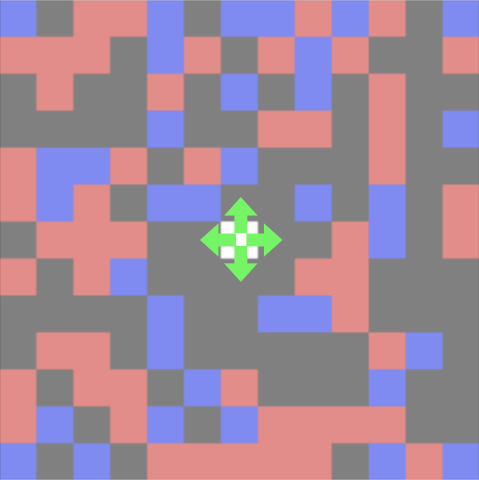
\includegraphics[width=5cm]{images/board.jpeg} 
%\begin{frame}[allowframebreaks]
  %      \frametitle{References}
    %    \bibliographystyle{amsalpha}
      %  \bibliography{biblio.bib}
%\end{frame}

\begin{frame}{En conclusion}

Quels outils pour le \textit{machine learning} ?

\begin{itemize}
\item des statistiques ;
\item de l'algèbre linéaire ;
\item de l'optimisation ;
\item de l'algorithmique ;
\item du Python ;
\item et beaucoup d'anglais !
\end{itemize}

\end{frame}

% python, anglais

\end{document}
